\documentclass[twoside,doctor]{zjnuthesis}
% 博士只需将上述一行的 master 改为 doctor
% ==============================================================
% ==============================================================

% 自己需要增加什么 package 或修改什么设置的话,都放在这里吧。
\usepackage{enumerate}
\usepackage{zhlipsum}
% \usepackage{etoc}
\usepackage{float}
\newcommand{\tabincell}[2]{\begin{tabular}{@{}#1@{}}#2\end{tabular}}

\allowdisplaybreaks
\raggedbottom

%%% ========================================================================== %%
%%% ============ 以下为封面内容,请根据实际情况填入 ========================== %%
%%% ========================================================================== %%


% === 中文封面内容 ===%
% \SchoolCode{10345}         %学校代码
\ResearchType{基础研究}    %研究类型
\Cfdlevel{国密}       %密级, 博士填写
\FirstDiscip{数学}    %一级学科, 博士填写
\SecDiscip{基础数学}    %二级学科, 博士填写
\ResearchDir{调和分析}	  %研究方向, 博士填写
\college{数学科学学院}     %所在学院, 博士填写
\Title{快速上手示例文档} %题目
\SubjectMajor{基础数学}                  %学科专业
\Grade{2020级}               %年级
\StudentID{66666666}     %学号
\Graduate{张三}             %作者
\Advisor{李四}             %指导教师
\Classification{O174.2}      %中图分类号
\SubmitDate{2023~年~6~月~6~日}     %硕士论文提交时间
\submitDate{2023~年~6~月~6~日}     %博士论文提交时间

% === 中英文扉面内容 ===%
\Title{快速上手示例文档} %
\EnglishTitle{\textsc{Quick Start and Document Snippets}}
% \upperTitle{$(q, r)$ BOUNDEDNESS OF ROUGH PSEUDO-DIFFERENTIAL OPERATORS}
\Author{张三}                               %作者
\EnglishAuthor{Zhang San}                  %英文作者
\Advisor{李四}                              %导师
\EnglishAdvisor{Li Si}                    %英文导师
\Major{基础数学}                              %专业
\EnglishMajor{Pure Mathematics}      %英文专业
\Degree{理学硕士}                                 %学位
\EnglishDegree{Master of Science}                       %英文学位
\Institute{浙江师范大学}                      %授予单位
\EnglishInstitute{Zhejiang Normal University} %英文授予单位

\begin{document}

% === 显示格式化封面 ===%
\maketitlecn

% === 显示格式化中英文扉面 ===%
\maketitleen

%% 把页码切换成罗马数字格式,并且不再对章进行自动编号
\frontmatter
% 
%%% ========================================================================== %%
%%% =========================== 摘要 ========================================= %%
%%% ========================================================================== %%
%% 中文摘要

\begin{Abstract}
  本文是 \ZJNUthesis 模板以及相关软件的简单使用说明,
  请大家仔细阅读该文件和 main.tex 主文件中的注释说明.
  请不要更改主文件的框架.
  如对本模板有任何建议,请以 ``数学模板: 问题简介'' 为题,发邮件给 allenryb@zjnu.edu.cn

  以下是随机生成内容, 用于测试
  
  \zhlipsum[1-5]

  \Keywords{模板; 测试; 使用说明}
\end{Abstract}

%% 英文摘要
\begin{EnglishAbstract}

  The followings is randomly generated for debug. 

  \zhlipsum[1-10]
  
  \EnglishKeywords{template; debug; tutorial}  
\end{EnglishAbstract}
% 
%%% ========================================================================== %%
%%% =========================== 目录 ========================================= %%
%%% ========================================================================== %%

\tableofcontents

% 
%%% ========================================================================== %%
%%% ========================= 正文部分 ======================================= %%
%%% ========================================================================== %%
%% 把页码切换成阿拉伯数字,并对章进行自动编号
\mainmatter

\chapter{快速上手}
\section{欢迎}

欢迎使用 \ZJNUthesis,本文档将介绍如何利用 \ZJNUthesis 模板进行学位论文写作,
假设读者有 \TeX 写作经验,并会使用搜索引擎解决常见问题。

通常说的 \TeX 包含了两部分:编译环境和编辑器。 

\section{\TeX 编译环境}

\TeX 编译环境往往包含了 \TeX 内核、必要程序、宏包等等编译必须的文件,
被集成在各个 \TeX 发行版中。
不同的发行版之间往往存在兼容性问题。
本模板采用了 texlive 发行版。
下面介绍在 Windows 中 texlive 的安装方式。
由于笔者没有 Mac 电脑,
所亚 Mac 电脑可根据实际情况进行。

\begin{enumerate}[1.]
\item 卸载以前装过的 \TeX 发行版,同时
  \textbf{检查系统环境变量和账户环境变量,确保其中不存在和 tex 相关的任何路径}。
  
\item 下载 texlive 安装包。
  在浏览器中输入
  \begin{quote}
    \url{https://tug.org/texlive/files/texlive2023-20230313.iso.torrent}
  \end{quote}
  下载 texlive 种子文件,并用迅雷、qBittorrent、transmission 等 BT 软件下载安装包。
  注意,texlive 安装包较大 (4-5G 左右),虽然有在线安装方式,但受限于网络带宽,
  我们建议先下载安装包。
  该安装包为 .iso 文件。
  
\item 打开安装包,运行 install-tl.bat 或者 install-tl-windows.bat。
  安装选项中,除安装路径外,其他都保持默认状态。建议安装路径选在固态硬盘中。
  安装时间根据电脑性能决定,需要 30 分钟 -- 8 小时不等。
  
\item 安装完毕后,再次检查系统环境变量或者账户环境变量,确保 texlive 的 bin 路径已在环境变量中。
  该路径在笔者的 Windows 电脑是 C:{\textbackslash}texlive{\textbackslash}2023{\textbackslash}bin{\textbackslash}windows
\end{enumerate}

\section{\TeX 编辑器}

在安装好 texlive 后,可用 Windows 自带的记事本软件配合命令行工具编写 \TeX 代码并输出 PDF。
\TeX 编辑器的目的是辅助我们更高效的输入 \TeX 代码并进行编译。
受限于笔者的经验和代码水平,\TeX 编辑器主要有以下几种 (以笔者的推荐程度排列):
\begin{itemize}
\item Emacs\textsc{+}AUCTEX 或者 Vim\textsc{+}VimTeX:最强编辑器之二,出色自定义能力,但需要一段学习时间
\item VSCode\textsc{+}LaTeX Workshop
\item TeXstudio 或者 Texmaker:\TeX 的专业编辑器,适合初学者
\end{itemize}

我们以 Texmaker 为例,简单介绍使用方法。
\begin{enumerate}[1.]
\item 从如下 Texmaker 官网中下载并安装 Texmaker
  \begin{quote}
    \url{https://www.xm1math.net/texmaker/}
  \end{quote}
  由于本模板需要用 xelatex 和 bibtex,所以我们要对 Texmaker 的快速编译按钮做设置。
  
\item 打开 Texmaker,依次进入
  \begin{quote}
    选项 \(\rightarrow\) 配置 Texmaker \(\rightarrow\) 快速构建
  \end{quote}
  
\item 在快速构建页面中,点选 User, 并点击图 \ref{fg:wizard} 按钮
  \begin{figure}[H]
    \centering
    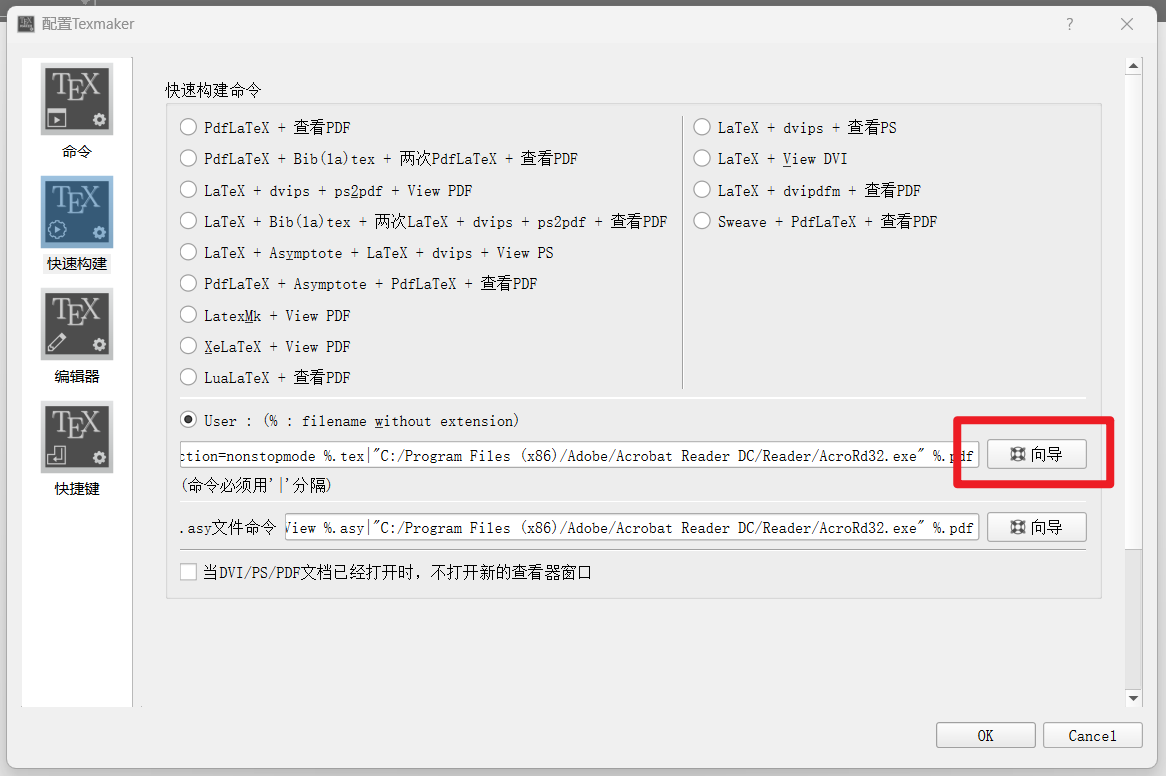
\includegraphics[width=.8\textwidth]{images/texmakerWizard.png}
    \caption{Texmaker 快速构建配置 1}
    \label{fg:wizard}
  \end{figure}
  
\item 在弹出菜单中,通过点选左边的命令,并用中间的添加按钮,使得右边如图 \ref{fg:quick} 所示
  \begin{figure}[H]
    \centering
    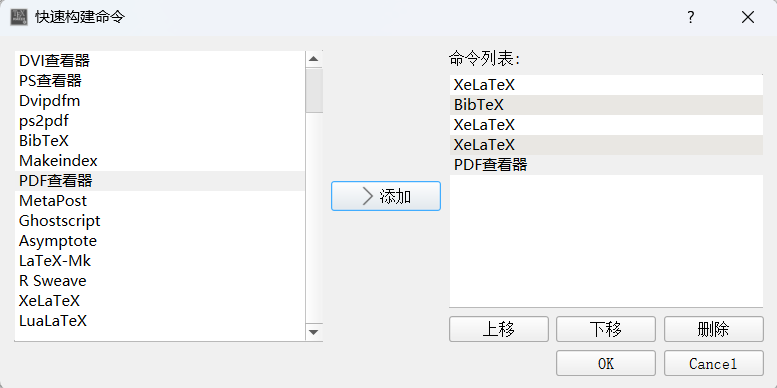
\includegraphics[width=.8\textwidth]{images/quickBuild.png}
    \caption{Texmaker 快速构建配置 2}
    \label{fg:quick}
  \end{figure}
  点击 OK 保存配置。
  
\item 输入 \TeX 代码,点击图 \ref{fg:button} 红框中的 ``快速构建'' 箭头来编译 \TeX 代码,点击 ``查看PDF'' 箭头查看 PDF.
  \begin{figure}[H]
    \centering
    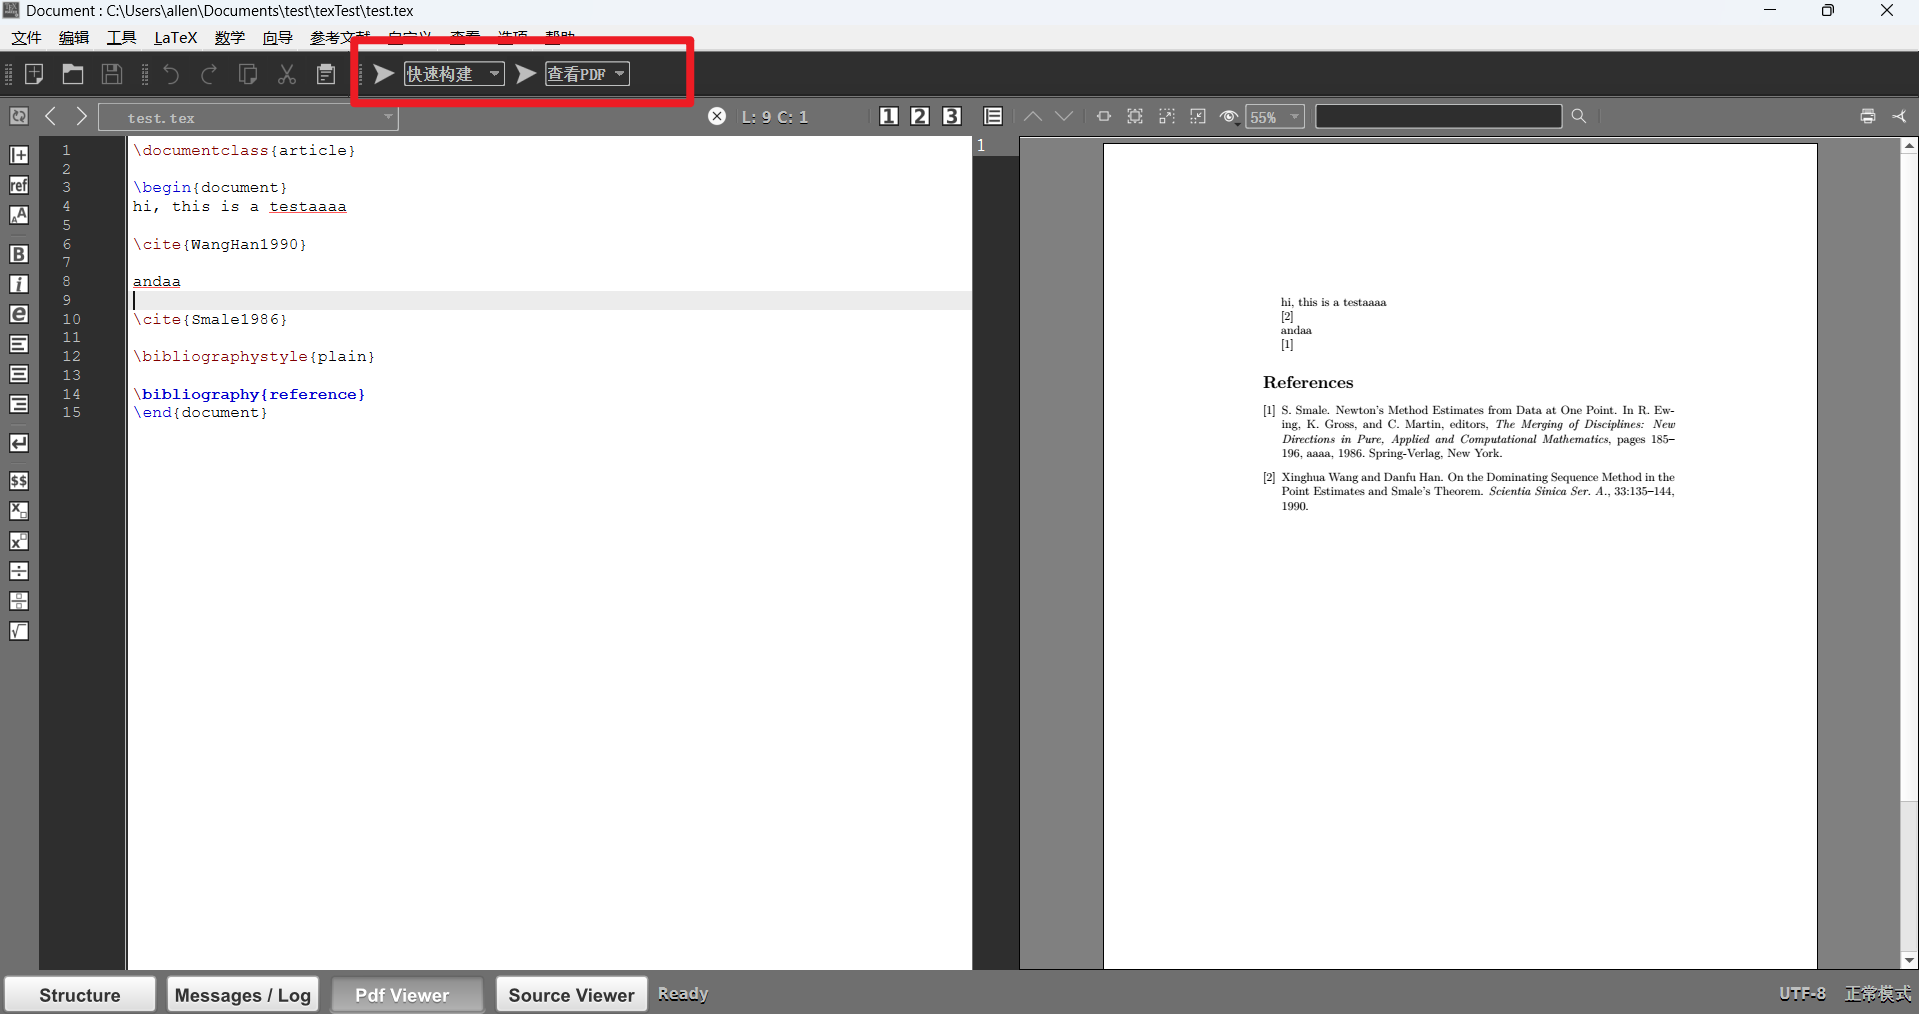
\includegraphics[width=.8\textwidth]{images/button.png}
    \caption{Texmaker 快速构建配置}
    \label{fg:button}
  \end{figure}
\end{enumerate}

以上是 Texmaker 的基本使用方法,该编辑器的其他辅助输入功能,留给大家自行探索。

\section{模板简介}

论文写作时,请确认\textbf{论文的目录}(main.tex所在的目录)下有以下文件:
\begin{itemize}
\item zjnuthesis.cls 文档必要的配置
\item logo 文件夹,内含学校的LOGO图标
\item preparations 文件夹,内含字体和论文声明类文件
\item main.tex,论文的主文件,请根据该文件中的注释输入 \TeX 代码,可修改文件名,但不可修改扩展名
\item reference.bib,请在该文件中输入参考文献。模板采用 bibtex 管理文献,
  会自动把文献按出现顺序排列,
  自动按照国标 GBT7714-2005 整理引用格式,
  自动根据第一行 \enquote{@} 后的字段 (article, book 等) 在每个文献标题后添加文献类型, 如 [J], [M] 等。
\end{itemize}

如果论文目录下没有这些文件的话,请从本模板根目录复制一份。
由于本模板涉及到中文和 bibtex,所以需要四次编译,顺序为
\begin{quote}
  xelatex \(\rightarrow\) bibtex \(\rightarrow\) xelatex \(\rightarrow\) xelatex
\end{quote}
如果采用上述 Texmaker 设置,那么只需采用快速编译即可。

博士论文封面和硕士论文略有不同。
\textbf{博士论文需将模版主文件 main.tex 第一行中的 master 替换为 doctor.}

\section{\TeX 基本语法}

对于不熟悉 \TeX 语法或者没有系统学习过 \TeX 语法的同学,可仔细阅读
《111 分钟了解 \LaTeXe》一书。此书可在文件夹 demos 找到。

本模板中已经加载了以下宏包:
\begin{itemize}
\item main.tex 包含了
  \begin{quote}
    enumerate, zhlipsum, lipsum, float
  \end{quote}
  
\item zjnuthesis.cls 包含了
  \begin{quote}
    \begin{flushleft}
      geometry, footmisc, xifthen, amsmath, amsthm, amsfonts, amssymb, mathrsfs, bm, ctex,
      times, fontenc, graphicx, graphics, epstopdf, fancyhdr, titlesec, titletoc,
      caption, nomencl, float, calc, indentfirst, algpseudocode, algorithm, tocbibind, tocloft,
      hyperref, lscape, longtable, booktabs, multirow, dcolumn, colortbl, threeparttable,
      array, natbib, tabularray, multicol, tasks, xcolor, tikz, ulem, setspace
    \end{flushleft}
  \end{quote}
\end{itemize}
很多包之间有兼容性问题。
大家可在 main.tex 中添加和修改所需的宏包。
由于 zjnuthesis.cls 中预加载的包决定了本模板的框架,
所以请审慎修改该文件中的包和参数。
如确需修改,请保证论文样式与本模板一致。

\section{注意事项}

由于 preparations 中加载的字体不包含粗体和斜体,
所以当前模版无法很好地实现这两个功能.
当前是以 AutoFakeBold 的形式来加载的, 实现程度较差. 下面是一些粗体的例子:

\begin{itemize}
\item 英文粗体测试 test, \textbf{test}

\item 中文粗体测试, \textbf{中文}

\item 数学字符粗体, \(\bm{\alpha}\)
\end{itemize}

建议尽量避免这两种字体应用. 





\chapter{简单示例}

这是第二章,目的是展示一些示例。

\section{看看第一节}

\subsection{图片示例}

附上照片一张图 \ref{fg:lake},来源 B 站。

\begin{figure}[H]
  \centering
  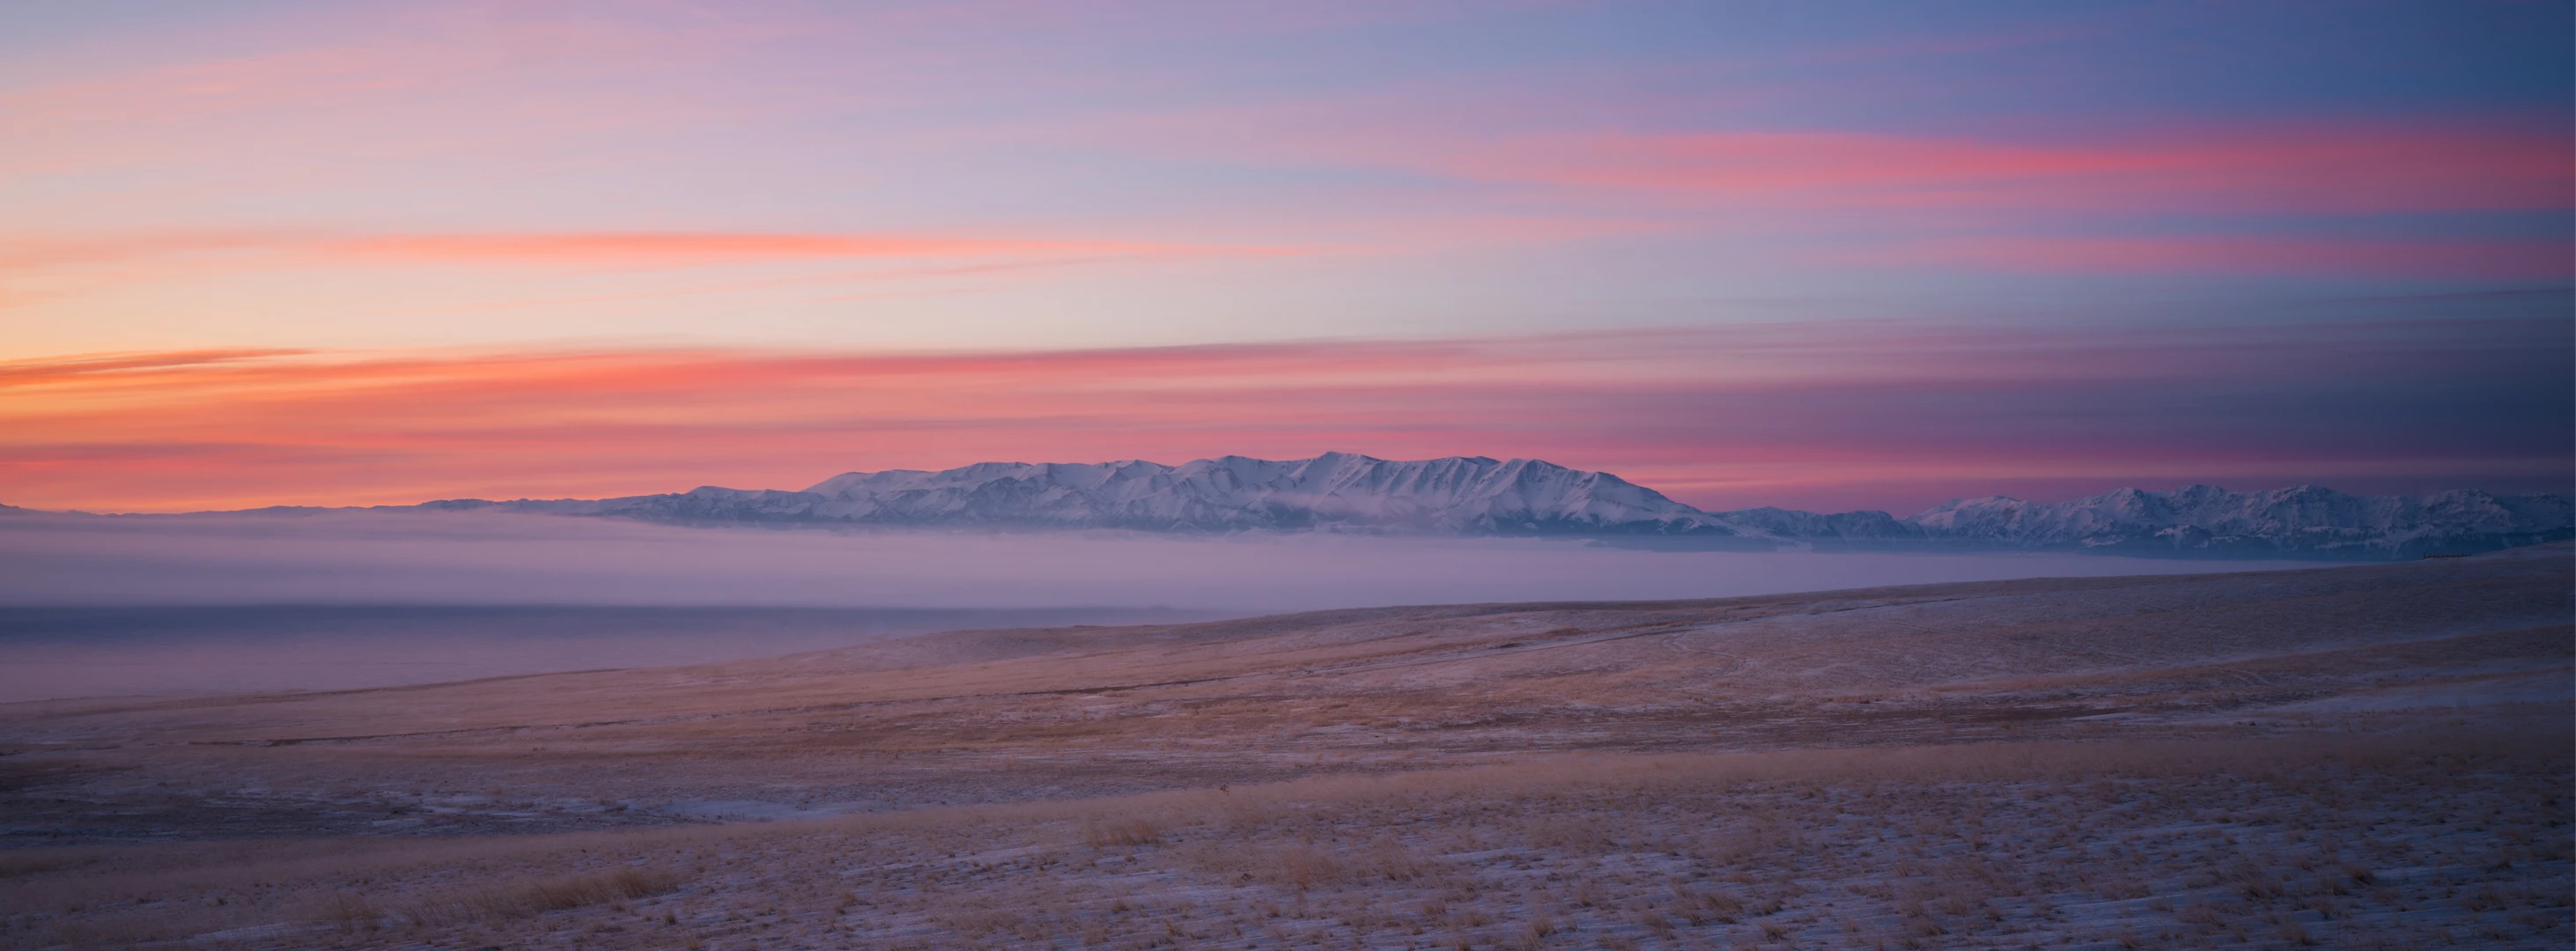
\includegraphics[width=.8\textwidth]{images/tangseng1.png}
  \caption{赛里木湖}
  \label{fg:lake}
\end{figure}


\subsection{表格示例}
\begin{table}[htb]
  \centering
  \caption{模板中的表格宏包}
  \label{tab:simple-table}
  \begin{tabular}{ll}
    \toprule
    \multicolumn{1}{m{20mm}}{\heiti\centering 宏包} & \multicolumn{1}{m{80mm}}{\heiti\centering 描述} \\
    \midrule
    longtable & 绘制跨页的表格。 \\
    booktabs & 三线表中的那三条线的命令来自这里。\\
    caption2 & 用于设置标题很方便,已经过时了,不过 \TeX Live 中还有。\\
    multirow & 跨行的单元格用这个宏包。\\
    dcolumn  & 想让表格小数点对齐吗?用这个宏包吧。\\
    \rowcolor[gray]{.9} colortbl & 表格上色。自己看着爽而已,打印出来都是黑白的。 \\
    threeparttable & 用来给表格添加脚注啥的很方便。 \\
    array & 忘了用来做什么了,但似乎很重要。 \\
    \bottomrule
  \end{tabular}
\end{table}

\subsection{定理等环境示例}

\begin{definition}
  这是定义环境
\end{definition}

\begin{theorem}
  这是带编号的定理环境
\end{theorem}

\begin{theorem*}
  这是没有编号的定理
\end{theorem*}
\begin{proposition}
  这是命题环境.
\end{proposition}

\begin{corollary}
  这是推论环境
\end{corollary}

\begin{proof}
  这是证明环境
\end{proof}

\begin{remark}
  这是带编号的注
\end{remark}

\begin{remark*}
  这是不带编号的注
\end{remark*}

\begin{proposition}
  天不言自高,水不言自流。
  \begin{gather*}
    \begin{split} 
      \varphi(x,z)
      &=z-\gamma_{10}x-\gamma_{mn}x^mz^n\\
      &=z-Mr^{-1}x-Mr^{-(m+n)}x^mz^n
    \end{split}\\[6pt]
    \begin{align} \zeta^0&=(\xi^0)^2,\\
      \zeta^1 &=\xi^0\xi^1,\\
      \zeta^2 &=(\xi^1)^2,
    \end{align}
  \end{gather*}
\end{proposition}


\subsection{公式示例}
贝叶斯公式如式 (\ref{equ:chap1:bayes}),其中 $p(y|\mathbf{x})$ 为后验;$p(\mathbf{x})$ 为先验;分母 $p(\mathbf{x})$ 为归一化因子。
\begin{equation}
  \label{equ:chap1:bayes}
  p(y|\mathbf{x}) = \frac{p(\mathbf{x},y)}{p(\mathbf{x})}=
  \frac{p(\mathbf{x}|y)p(y)}{p(\mathbf{x})} 
\end{equation}
论文里面公式越多,\TeX 就越 happy。再看一个 \textsf{amsmath} 的例子:
\newcommand{\envert}[1]{\left\lvert#1\right\rvert} 
\begin{equation}\label{detK2}
  \det\mathbf{K}(t=1,t_1,\dots,t_n)=\sum_{I\in\mathbf{n}}(-1)^{\envert{I}}
  \prod_{i\in I}t_i\prod_{j\in I}(D_j+\lambda_jt_j)\det\mathbf{A}
  ^{(\lambda)}(\overline{I}|\overline{I})=0.
\end{equation} 
大家在写公式的时候一定要好好看 \textsf{amsmath} 的文档,并参考模板中的用法:
\begin{multline*}\tag{[b]} 
  \int_a^b\biggl\{\int_a^b[f(x)^2g(y)^2+f(y)^2g(x)^2]
  -2f(x)g(x)f(y)g(y)\,dx\biggr\}\,dy \\
  =\int_a^b\biggl\{g(y)^2\int_a^bf^2+f(y)^2
  \int_a^b g^2-2f(y)g(y)\int_a^b fg\biggr\}\,dy
\end{multline*}
其实还可以看看这个多级规划:
\begin{equation}\label{bilevel}
  \left\{
    \begin{array}{l}
      \displaystyle \max_x F(x,y_1^*,y_2^*,\cdots,y_m^*)\\[0.2cm]
      \mbox{subject to:}\\[0.1cm]
      \qquad G(x)\le 0\\[0.1cm]
      \qquad(y_1^*,y_2^*,\cdots,y_m^*)\mbox{ solves problems }(i=1,2,\cdots,m)\\[0.1cm]
      \qquad\left\{\begin{array}{l}
                     \displaystyle \max_x f_i(x,y_1,y_2,\cdots,y_m)\\[0.2cm]
                     \mbox{subject to:}\\[0.1cm]
                     \qquad g_i(x,y_1,y_2,\cdots,y_m)\le 0.
                   \end{array}\right.
    \end{array}\right.
\end{equation}

\section{参考文献}

如前所述,本模板用 bibtex 管理参考文献, 会自动把文献按出现顺序排列,
自动按照国标 GBT7714-2005 整理引用格式,
自动根据第一行 \enquote{@} 后的字段 (article, book 等) 在每个文献标题后添加文献类型, 如 [J], [M] 等。
具体文件见 \texttt{reference.bib}。
关于 bibtex 的格式,可参见
\begin{quote}
  \url{https://www.overleaf.com/learn/latex/Bibliography_management_with_bibtex}
\end{quote}
以下是部分参考文献的例子: 
\cite{Smale1986}, \cite{WangHan1990}, \cite{Deuflhard2004}, \cite{test2004} 和
\cite{WangHan2000}, 
\cite{WangHan2001}, 
\cite{WangHan2002}, 
\cite{WangHan2003}, 
\cite{WangHan2004}, 
\cite{WangHan2005}, 
\cite{WangHan2006}, 
\cite{WangHan2007}, 
\cite{WangHan2008}, 
\cite{WangHan2009}, 
\cite{WangHan2010}, 
\cite{WangHan2011}, 
\cite{WangHan2012}, 
\cite{WangHan2013}, 
\cite{WangHan2014}, 
\cite{WangHan2015}, 
\cite{WangHan2016}, 
\cite{WangHan2017}, 
\cite{WangHan2018}, 
\cite{WangHan2019}, 
\cite{WangHan2020}, 
\cite{WangHan2021}

参考文献中的两个自动信息:
\begin{itemize}
\item 如果参考文献列表中出现 \enquote{[S.l.]}, 那么对应的文献需补充 \enquote{出版地}.
  
\item 如果参考文献列表中出现 \enquote{[s.n.]}, 那么对应的文献需补充 \enquote{出版社}.
\end{itemize}

%% 它不再对章进行自动编号,但不改变页码数字格式,不重设页码计数器
\backmatter

%%% ========================================================================== %%
%%% ========================= 参考文献 ======================================= %%
%%% ========================================================================== %%
% 模板会自动把文献按出现顺序排列
% 模板会自动按照国标 GBT7714-2005 整理引用格式
% 自动根据第一行 "@" 后的字段 (article, book 等) 在每个文献标题后添加文献类型, 如 [J], [M] 等

% \chaptermark{参考文献}
% \addcontentsline{toc}{chapter}{参考文献}
% 解决目录中没有相应的参考文献的条目问题
\bibliography{reference}

%%% ========================================================================== %%
%%% =========================== 附录 ========================================= %%
%%% ========================================================================== %%

\chapter{附录~~比较定理}

请根据需要修改.
不需要附录的使用者,请注释掉这部分。

%%% ========================================================================== %%
%%% =========================== 致谢 ========================================= %%
%%% ========================================================================== %%

\chapter{致谢}

感谢父亲母亲等等。
对导师和给予指导或协助完成学位论文工作的组织和个人表示感谢。内容应简洁明了、实事求是。对课题给予资助者应予感谢。

%%% ========================================================================== %%
%%% ======================= 发表文章目录 ===================================== %%
%%% ========================================================================== %%

%% 攻读学位期间取得的研究成果

\chapter{攻读学位期间取得的研究成果}

\begin{enumerate}[{[}1{]}]
\item 阮高峰,徐晓东. OpenID分布式身份认证系统及其教育应用展望[J].中国电化教育,2008(10):55-59.

\item 马克·J·罗森伯格.在线学习:强化企业优势的知识策略[M]. 北京:机械工业出版社, 2002:19-22.

\end{enumerate}

%%% ========================================================================== %%
%%% =============== 承诺书、独创性声明、授权声明 ============================= %%
%%% ========================================================================== %%
% 不要修改以下内容
%%% ========================================================================== %%
%%% ============== 浙江师范大学学位论文诚信承诺书 ============================ %%
%%% ========================================================================== %%

%% 诚信承诺书
\chapter*{浙江师范大学学位论文诚信承诺书}
\addcontentsline{toc}{chapter}{浙江师范大学学位论文诚信承诺书}

{\xiaosan\linespread{1.5}\selectfont
  我承诺自觉遵守《浙江师范大学研究生学术道德规范管理条例》。我的学位论文中凡引用他人已经发表或未发表的成果、数据、观点等,均已明确注明并详细列出有关文献的名称、作者、年份、刊物名称和出版文献的出版机构、出版地和版次等内容。论文中未注明的内容为本人的研究成果。

  如有违反,本人接受处罚并承担一切责任。      

  \vspace{20pt}
  \begin{flushright}
    承诺人(研究生): \phantom{\hspace{100pt}} \\[20pt]
    指导教师: \phantom{\hspace{100pt}}
  \end{flushright}
}


%%% ========================================================================== %%
%%% ========= 学位论文独创性声明和学位论文使用授权声明 ======================= %%
%%% ========================================================================== %%

%% 以下这四行代码是在该页面之前加入一页空白页!!
% \newpage
% \thispagestyle{empty}
% \
% \newpage

\begin{flushleft}
  \begin{minipage}{15cm}
    \begin{OriginalityStatements}
      \setlength{\parindent}{2em}\xiaosi
      本人声明所呈交的学位论文是我个人在导师指导下进行的研究工作及取得的研究成果。论文中除了特别加以标注和致谢的地方外,不包含其他人或其他机构已经发表或撰写过的研究成果。其他同志对本研究的启发和所做的贡献均已在论文中作了明确的声明并表示了谢意。本人完全意识到本声明的法律结果由本人承担。
      \newline
      \newline

      \noindent
      作者签名:\hspace*{60pt}
      \hfill
      日期:\hspace*{40pt}2025
      年  \hspace*{20pt}6
      月  \hspace*{20pt}10 日
    \end{OriginalityStatements}

    \vspace{20ex}
    
    \begin{LicenseStatements}
      \setlength{\parindent}{2em}\xiaosi
      本人完全了解浙江师范大学有关保留、使用学位论文的规定,即:学校有权保留并向国家有关机关或机构送交论文的复印件和电子文档,允许论文被查阅和借阅,可以采用影印、缩印或扫描等手段保存、汇编学位论文。同意浙江师范大学可以用不同方式在不同媒体上发表、传播论文的全部或部分内容。
      
      保密的学位论文在解密后遵守此协议。
      \newline
      \newline

      \noindent
      作者签名:\hspace*{60pt}
      导师签名:\hfill
      日期:\hspace*{40pt}2025
      年 \hspace*{20pt}6
      月 \hspace*{20pt}10 日

    \end{LicenseStatements}
  \end{minipage}
\end{flushleft}

\end{document}

%%% Local Variables: 
%%% coding: utf-8
%%% mode: latex
%%% TeX-engine: xetex
%%% End: 
